\section{Introduction}\label{sec:intro}

In the five cancer-predisposition genes studied here, 81\% of the ClinVar missense records classified as (likely)
pathogenic, (likely) benign or uncertain are variants of uncertain significance (VUS) \cite{Landrum2018}, and for many of them computational
predictors are among the few sources of evidence \cite{Pejaver2022}. The guidelines of the American College of Medical Genetics and
Genomics and the Association for Molecular Pathology (ACMG/AMP) grade evidence qualitatively \cite{Richards2015}; their Bayesian adaptation equates each strength with a likelihood ratio, the odds of
pathogenicity (OddsPath) \cite{Tavtigian2018,Brnich2020}, so the strength of a predictor's evidence is a statistical
estimate. Calibration workflows report it as a point estimate or a resampling-based bound
\cite{Pejaver2022,Bergquist2025,Badonyi2025}. When the calibration is specific to a gene, few labelled variants are
available and the threshold that defines the evidence is chosen from the same data; none of these bounds carries a
finite-sample guarantee that holds after this choice.

Two features of the data make the estimate fragile. First, the share of damaging variants (the prevalence) differs
between calibration sets and the variants being classified, and is unknown for the latter: in our five genes, 45\% of
confidently labelled ClinVar missense variants are pathogenic, whereas 6.0\% to 25.9\% of the other assayed missense
variants lose function in saturation genome editing (SGE) or deep mutational scanning (DMS) experiments
(\cref{tab:data}). Thresholds that depend on the class balance of the calibration set inherit this mismatch: calibrated
on assay data at a 5\% LoF share, marginal conformal thresholds covered the LoF variants of one gene--predictor pair at
only 0.11 (\cref{sec:coverage}). Second, gene-level labelled sets are small and substitutions at one residue are
dependent: in a resampling design with known truth, percentile-bootstrap bounds were respected in only 76.5\% of
threshold selections, and evidence levels claimed from point estimates held in only 79.7\% of claims
(\cref{sec:evidence}).

We introduce \textsc{CertiVar} (\cref{fig:overview}), which turns a predictor score into loss-of-function (LoF),
functional or no calls. Per-class (Mondrian) conformal thresholds set from SGE or DMS labels bound how often each class
is mis-called, and a certification step bounds the likelihood ratio of each call type with respect to the assay outcome,
valid after a threshold has been selected; neither needs an estimate of the LoF share. The certified quantity is how
strongly a call predicts the assay result; it is evidence about pathogenicity only to the extent that the assay is
clinically validated.

\begin{figure}[t]
\centering
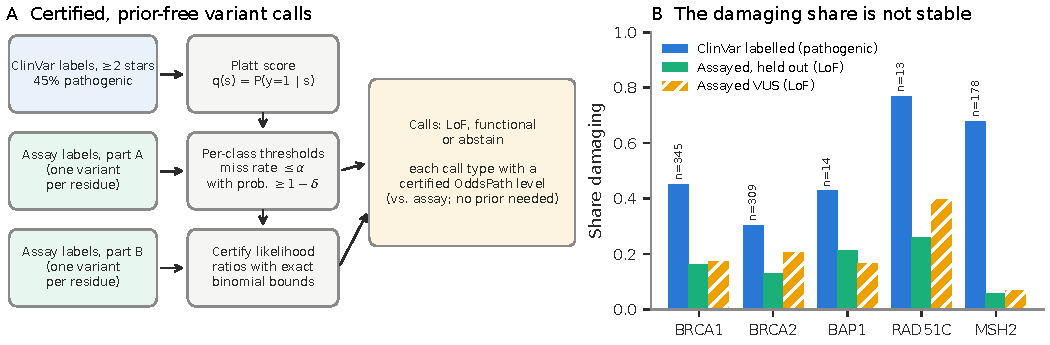
\includegraphics[width=\linewidth]{fig_overview.pdf}
\caption{\textsc{CertiVar}. Per-class thresholds are set on part $\mathcal A$ of a gene's assayed residues, and the
likelihood ratio of each call type with respect to the assay outcome is certified on a disjoint part $\mathcal B$; the
thresholds are then applied to the target variants. The grey path (Platt scaling on ClinVar labels) only puts
predictors on a common scale; it is a monotone map that does not change any call.}\label{fig:overview}
\end{figure}

Our contributions are as follows. (1) We formulate predictor-based calling as abstaining classification with per-class
error control on residue-clustered data, and prove that the certified likelihood-ratio bounds hold after selection from
a grid of thresholds, that per-class coverage after the selection is at least one minus the largest grid level, and that a fixed-sequence
variant certifies a
level without a multiplicity correction over the grid (\cref{sec:method}). (2) In a known-truth resampling design,
exact binomial bounds on one variant per residue held where bootstrap bounds and point estimates often did not, and the
fixed-sequence variant certified moderate evidence more than twice as often as the Bonferroni correction
(\cref{sec:evidence}).
(3) On five genes and three predictors, per-class coverage stayed at the target when the calibration LoF share ranged
from 5\% to 50\%, where marginal and prior-reweighted conformal prediction failed, and held approximately on assayed VUS
(\cref{sec:coverage,sec:shift}). (4) We quantify the cost and the limits: mostly supporting-level evidence, abstention
on about a third of variants or more, the need for same-gene assay data, and weaker certificates in held-out protein
regions (\cref{sec:transfer}).
